
\subsection{Single Burst}

For a stellar population that forms impulsively, the rate of mass and energy injection per unit stellar mass at age $t$ are given, respectively, by 
\begin{align} 
  \dot{\bar{m}}(t) &= \frac{\Delta M(t) \mu|_{M_{\rm TO}(t)}
    \left|\dot{M}_{\rm TO}(t)\right| + f_{\rm MS} \int_{m_0}^{m_{\rm
        T}(t)}
    \dot{m}(\Mstar, t) \mu|_{\Mstar} {\rm d}\Mstar }{\bar{m}_*}\\
  \dot{\bar{e}}(t) &=\dot{e}_{\rm TO}(t)+ f_{\rm MS} \int_{m_0}^{m_{\rm T}(t)}
  \frac{\vw^2(\Mstar, t) \dot{m}(\Mstar, t) \mu|_{\Mstar} {\rm d}\Mstar}{\bar{m}_*},
  \label{eq:edotImp}
\end{align} 
where the first and second terms in each expression corresponds to
contributions from main sequence (MS) stars and post-main sequence
(PMS) stars, respectively.  Here $ f_{\rm MS} < 1$ is the efficiency
with which main sequence winds thermalize their energy with the rest
of the injected gas (we hereafter assume $f_{\rm MS} = 1$) and $\mu$
is the IMF, which we take to be of the Salpeter form $\mu|_{\Mstar}
\propto M_{\star}^{-2.35}$, truncated at $m_0 = 0.1 \Msun$ on the low
mass end and at $100 \Msun$ on the high mass end, where $\bar{m}_*$ =
0.35 $\Msun$ is the corresponding mean stellar mass.  Our optimistic
assumption of 100 per cent thermalization efficiency of stellar winds
is at least partially offset by our conservative assumption to neglect
energy input from core collapse supernovae, which contribute a
comparable energy injection rate to massive stellar winds.

The quantity of mass lost in PMS winds $\Delta M(t)$ is estimated from
the expression given by \citet{CiottiOstriker:2007a} (their eq.~[10]),
\begin{align}
\Delta M=
\begin{cases}
0.945 M_{\rm TO}-0.503 & M_{\rm TO} < 9 \Msun\\
 M_{\rm TO}-1.4 \Msun &  M_{\rm TO} \ge 9 \Msun,
\end{cases}
\end{align}
where $M_{\rm TO}$ is the turn-off mass, which at time $t < t_{\rm h}$ is calculated as
\begin{align}
\log(M_{\rm TO})/M_{\odot} =0.24 + 0.068 x^2-0.34 x+4.76 e^{-4.58 x},
\end{align}
where $x=\log(t/10^9 {\rm years})$.  This functional fit is designed
to reproduce the results of \citet{MaederMeynet:1987a} (their Table 9)
for massive stars while asymptoting to the formula provided by
\citet{CiottiOstriker:2007a} (their eq.~[9]) for intermediate and late
times ($t \gsim 10^8$ years).

{\bf AG: Go back to the old mass loss prescription ASAP so that we don't
  violate mass conservation!}
The MS wind mass loss rate $\dot{m}(\Mstar, t)$ is calculated based on
the generalization of Reimer's law given in
\citet{SchroderCuntz:2005a} (their eq.~[4]) as
\begin{align}
  \dot{m}=8 \times 10^{-14} \frac{L_* R_*}{\Mstar}
  \left(\frac{T_{\rm eff}}{\rm 4000 K}\right)^{3.5}
  \left(1+\frac{g_{\odot}}{4300 g_*}\right) \Msun \pyear,\
\end{align}
where  $R_*$, $L_*$, $T_{\rm eff}$ and $g_*$ are the stellar radius,
luminosity, effective temperature, and surface gravity, respectively, the latter normalized to its solar value $g_{\odot}$.  The stellar radius and luminosity are estimated as (\citet{Kippenhahn&Weigert90}; Figs.~22.2) 22.3)
\begin{align}
L_*=
\begin{cases}
L_{\odot} (\Mstar/\Msun)^{3.2} & \Mstar > \Msun \\
L_{\odot} (\Mstar/\Msun)^{2.5} & \Mstar \le \Msun
\end{cases}
\end{align}
\begin{align}
R_*=
\begin{cases}
R_{\odot} (\Mstar/\Msun)^{0.57} & \Mstar > \Msun \\
R_{\odot} (\Mstar/\Msun)^{0.8} & \Mstar \le \Msun
\end{cases}
\end{align}
The wind velocity of main sequence winds is assumed
to equal $v_w (\Mstar, t) = v_{w,\odot}(M_{\star}/M_{\odot})^{1/2}(R_{\star}/R_{\odot})^{-1/2}$, i.e.~scaling as the stellar escape velocity and normalized to the velocity of the solar wind $v_{w,\odot} = 430$ km s$^{-1}$; this produces an effective wind heating velocity for main
sequence winds alone of $\sim 100$ km s$^{-1}$ for $\tau_{\star} \sim t_{\rm h}$, close to the value found by \citet{NaimanSoares-Furtado+:2013a} for globular clusters based on a more
sophisticated population synthesis treatment. 

The rate of energy input from PMS winds, $\dot{e}_{\rm TO}(t) = f_{8}\dot{\mathcal{E}}/\bar{m}_*$, is dominated by fast Wolf-Rayet winds and core-collapse supernovae from massive stars ($M_{\star} > 8M_{\odot}$), where $f_{8} =2.6 \times 10^{-3}$ is the fraction of the stellar mass with $M_{\star} > 8M_{\odot}$ for our assumed Salpeter IMF.  Here $\dot{\mathcal{E}} (t)$ is the energy injection rate per massive star, which we estimate as
\begin{align}
\dot{\mathcal{E}} (t)=  1.3 \times 10^{36} {\rm erg\,s^{-1}}
\begin{cases}
  1 & t<4 \times 10^6 {\rm yr}\\
  \left(\frac{t}{4 \times  10^6\,{\rm yr}}\right)^{-3.73} & t \ge 4 \times 10^6 {\rm yr},
\end{cases}
\label{eq:voss}
\end{align}
based on the results of \citet{VossDiehl+:2009a} (their Fig.~7, top panel), who use a population synthesis code to simulate the mass and energy injection into the ISM from an OB association.  Although equation~\eqref{eq:voss} is valid only for $t \lsim 10$ Myr, in practice the precise functional form of $\dot{e}_{\rm TO}(t)$ is generally unimportant for our purposes, so we adopt equation~\eqref{eq:voss} as being valid for all times.


The effective wind velocity in the limit of an impulsive star formation may then be written
as 
\begin{align}
\bar{v}_w(t)=2 \dot{\bar{e}}(t)/\dot{\bar{m}}(t)
\label{eq:vwImp}
\end{align}
while 
\begin{align}
\eta = \dot{\bar{m}}(t) \th
\label{eq:etaImp}
\end{align}
 Figure~\ref{fig:vwImp} shows the values of $\bar{v}_w(t)$ and $\eta(t)$ as a function of stellar age, $\tau_{\star}$.

\begin{figure}
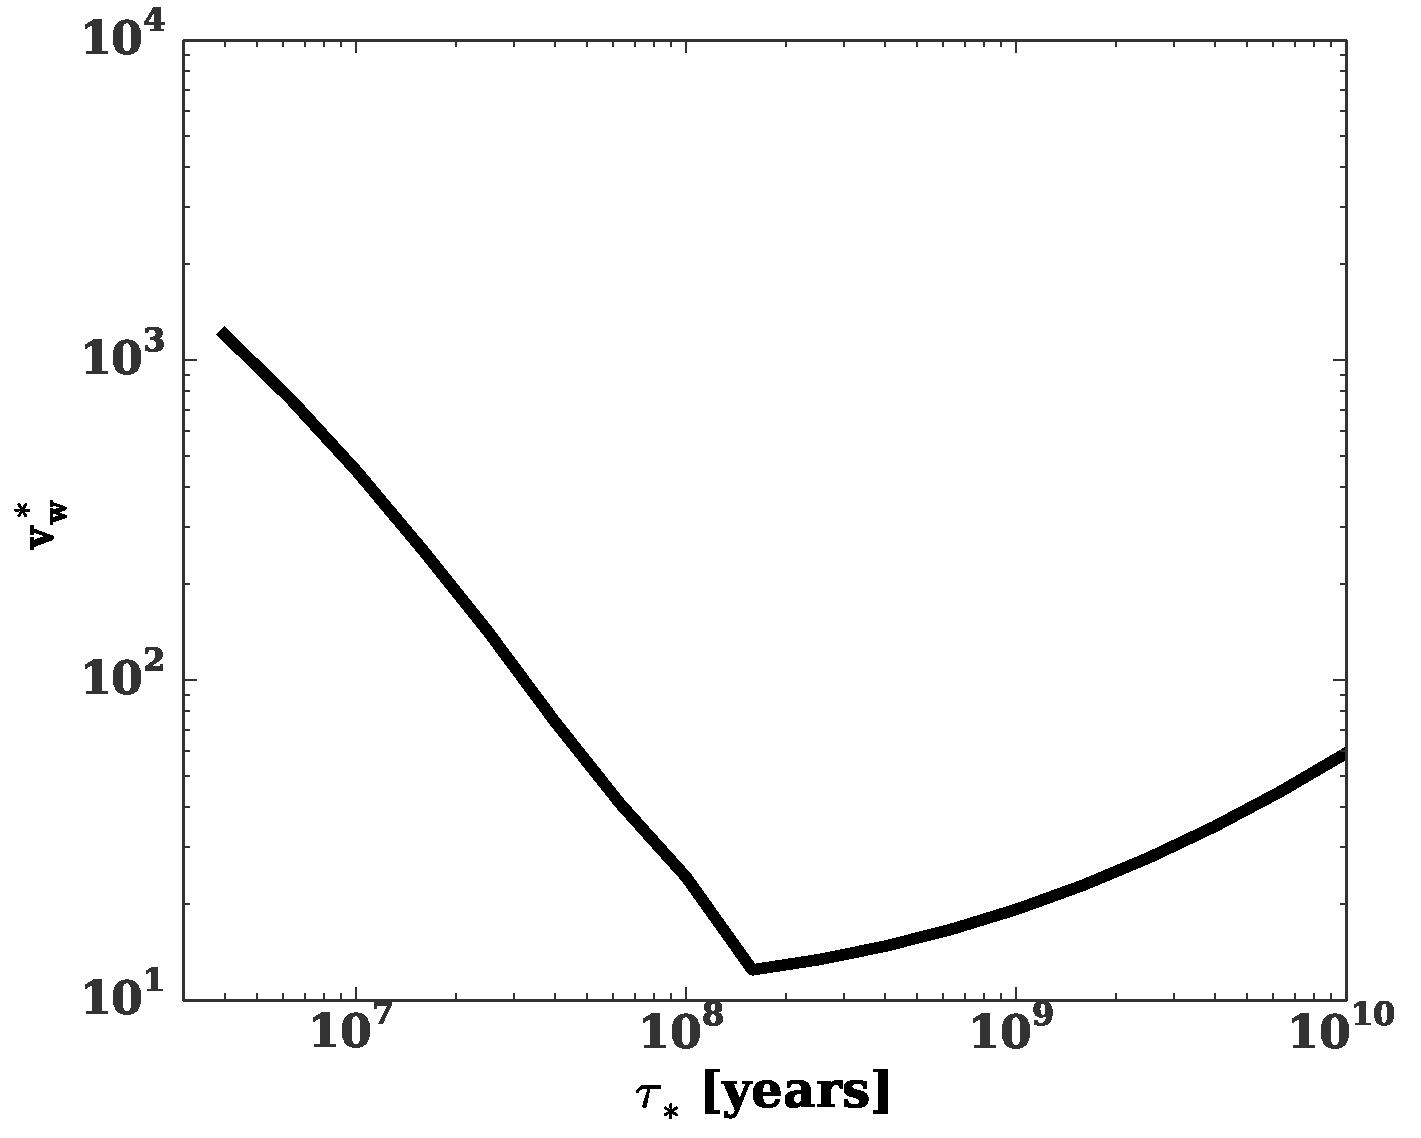
\includegraphics[width=\columnwidth]{vwImp.pdf}
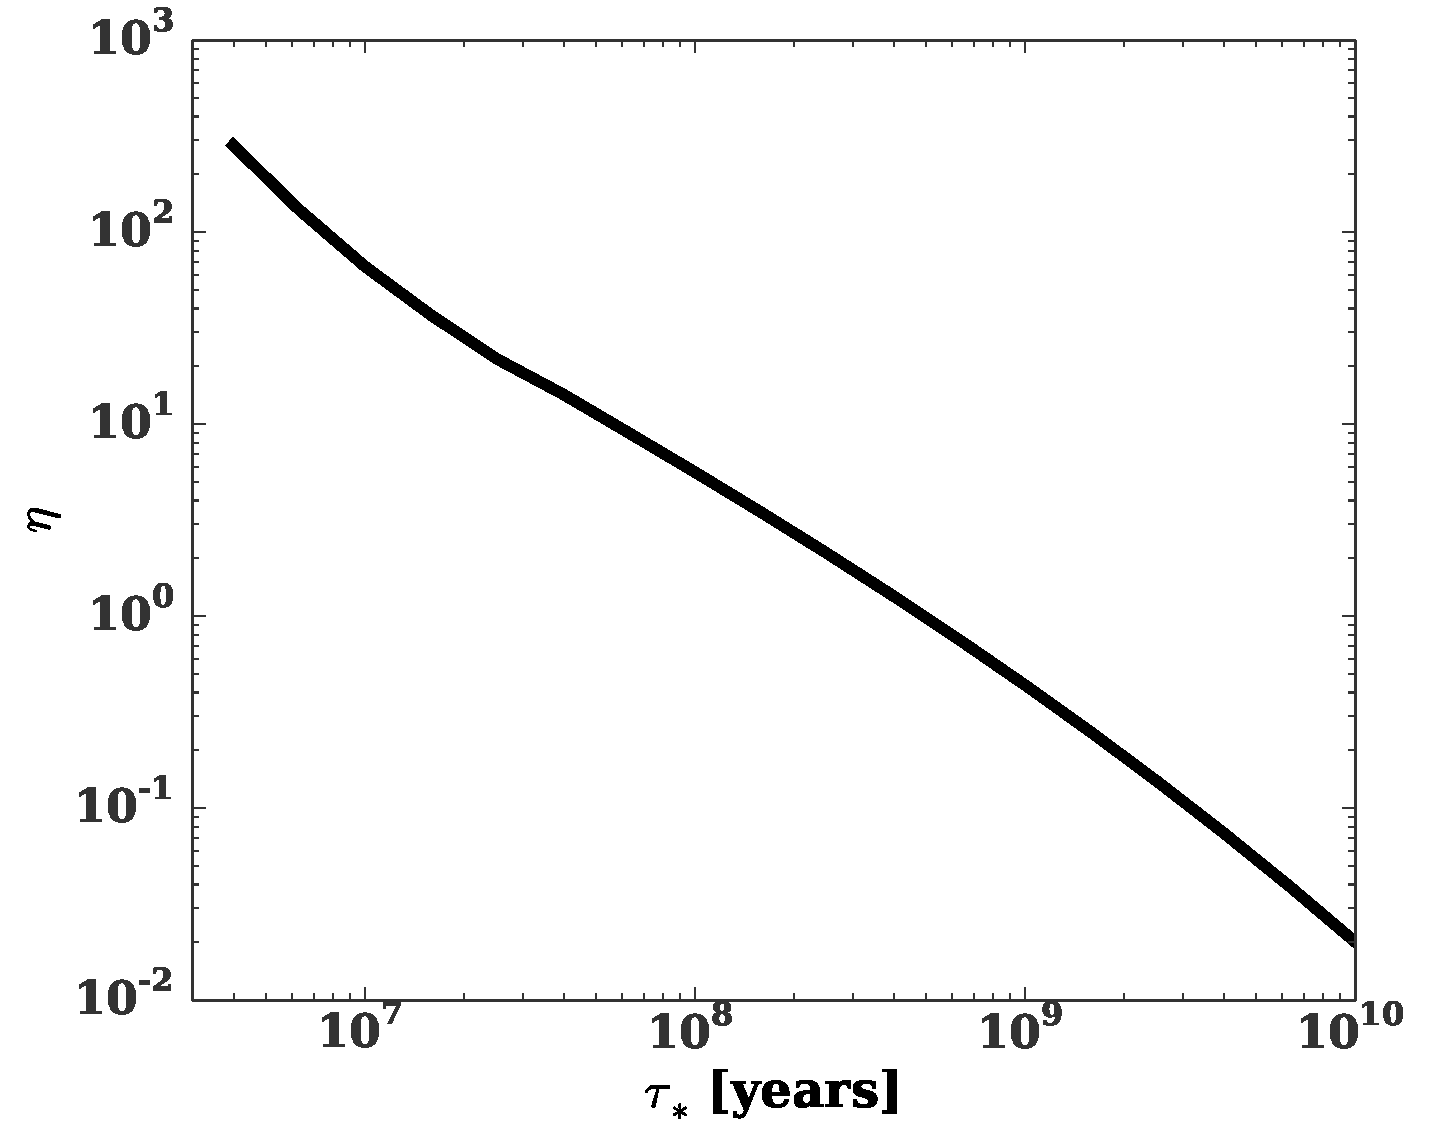
\includegraphics[width=\columnwidth]{etaImp.pdf}
\caption{\label{fig:vwImp} Effective heating rate, $v_w^{\star}$, and mass loss parameter, $\eta$ (eq.~[\ref{eq:q}]), resulting from stellar winds from a stellar population of age $\tau_{\star}$.}
\end{figure}



\subsection{Over Star Formation History}
Generalizing to an arbitrary star formation history $S(t)$, the total rate of mass and energy input can be written as
\begin{align} 
  \dot{M}(t) &= \int_0^t S(t_1) \dot{\bar{m}}(t-t_1){\rm
      d}t_1 \label{eq:MDotSFH}\\
  \dot{E}(t) &= \int_0^t S(t_1) \dot{\bar{e}}(t-t_1){\rm
      d}t_1, \label{eq:EDotSFH}
\end{align}
resulting in a wind heating parameter of 
\begin{align}
  v_w^2(t) &=2 \dot{E}(t)/\dot{M}(t).
\end{align}
The mass return parameter will be
\begin{align}
\eta = \frac{\dot{M}(t)}{\int_0^t S(t_1) {\rm d}t_1} \th
\end{align}

 \begin{figure}
  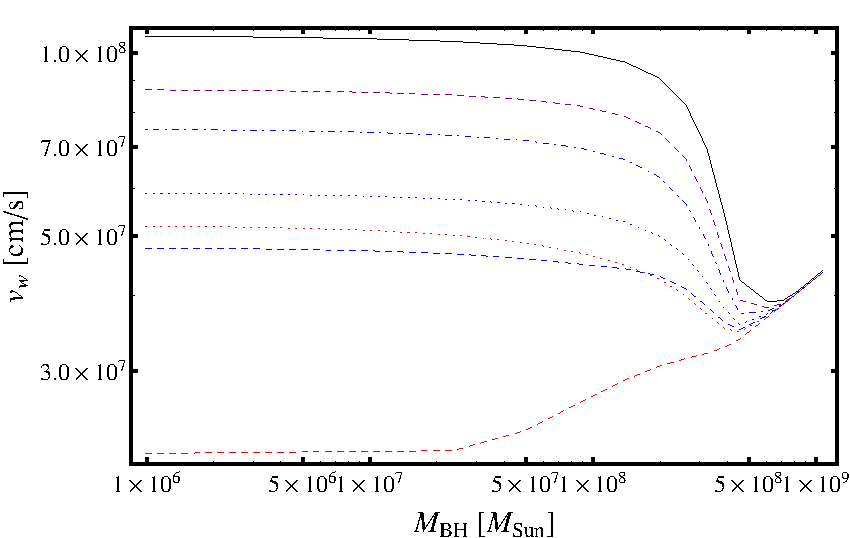
\includegraphics[width=\columnwidth]{NickPlot2.pdf}
  \caption{\label{fig:NickPlot2} Effective wind velocities for nonstandard
    star formation histories.  The black curve shows, for reference,
    $v_{\rm w}$ calculated using the halo-averaged $S(t)$.  Other
    colors show the effective wind velocities $\mathcal{V}_{\rm w}$
    computed using convolved star formation histories
    $\mathcal{S}(t)$.  The purple curve shows a recent drop in the
    star formation rate, i.e. $\delta t_{\star}=10^6~{\rm yr}$.  The blue
    and red curves show $\delta t_{\star}=10^7~{\rm yr}$ and $t_{\rm
      scale}=10^8~{\rm yr}$, respectively; longer scale times look
    quite similar to the red curves.  Dashed, dotted, and dot-dashed
    line styles show star formation rates that have declined to
    fractions $\iota= 0.001$, $\iota = 0.1$, and $\iota = 0.3$ of
    their halo-averaged values, respectively. }
  \end{figure}
  We estimate the stellar wind heating provided by the {\it average}
  star formation history of galaxies of a given $\Mbh$ using the
  results of \citet[eqs.~17-20]{MosterNaab+:2013a}.  Note that the
  star formation histories in \citet{MosterNaab+:2013a} are in terms
  of halo mass. For a given $\Mbh$ we assign the halo mass whose star
  formation history would produce a bulge consistent with the
  $\Mbh-M_{\rm bulge}$ relationship from \citet{McConnellMa:2013a}.  A
  slight complication occurs for the largest mass halos, where much of
  the $z=0$ stellar mass has been acquired through accretion of
  satellite halos rather than {\it in situ} star formation.  To
  accomodate this, we incorporate analytic fits for mass accretion
  histories, taken from \citet[their eqs.~21-23]{MosterNaab+:2013a},
  assuming that the age distribution of the accreted stars is equal to
  the age distribution of those formed {\it in situ}.  This assumption
  may be conservative if the primary galaxy's accretion history is
  dominated by minor mergers with younger stellar populations.  On the
  other hand, the dynamical friction inspiral time for small satellite
  galaxies is quite long, generally much greater than the $\sim
  10^7~{\rm yr}$ for which young stars can dominate the heating
  budget.  

To find the total mass ($\Mdot'(t)$) and energy
  ($\dot{E}'(t)$) injection rates, including the contribution of
  accreted stars, we add a convolution of the specific mass and
  injection rates with the accretion history $A(t)$ to the mass and
  energy injection rates from star formed in-situ.  Thus,

\begin{align}
\Mdot '(t)&=\Mdot(t)+\int_{0}^{t} A(t_{\rm acc}) \frac{\Mdot(t_{\rm acc})}
{\int_{0}^{t_{\rm acc}} S(t_1) dt_1} {\rm dt_{ acc}}\\
\dot{E}'(t)&=\dot{E}(t)+\int_{0}^{t} A(t_{\rm acc}) \frac{\dot{E}(t_{\rm acc})}
{\int_{0}^{t_{\rm acc}} S(t') dt_1} {\rm dt_{acc}}.
\end{align}

The corresponding wind heating parameter $v_w'$ and mass return
parameter, $\eta'$, will be given by

\begin{align}
\eta'&=\frac{\Mdot'(t)}{\int_0^t S(t_1) {\rm d}t_1+\int_0^t A(t_1) {\rm
    d}t_1} \th\\
v_w'^2&=2 \frac{\dot{E}'(t)}{\Mdot'(t)}.
\end{align}

Figure \ref{fig:NickPlot2} shows how the wind heating varies as star formation histories deviate from their halo-averaged values.  In particular, we show
\begin{align} 
  \dot{\mathcal{M}}(t) &= \int_0^t \mathcal{S}(t_1) \dot{\bar{m}}(t-t_1){\rm
      d}t_1\\
  \dot{\mathcal{E}}(t) &= \int_0^t \mathcal{S}(t_1) \dot{\bar{e}}(t-t_1){\rm
      d}t_1,\\
  \mathcal{V}_w^2(t) &=2 \dot{\mathcal{E}}(t)/\dot{\mathcal{M}}(t).
\end{align}
In these equations, 
\begin{equation}
\mathcal{S}(t) = S(t) \times \left(\frac{2}{\pi}(1-\iota)\arctan(t/\delta t_{\star}) + \iota \right).
\end{equation}
This function convolves the recent ($z \approx 0$) halo-averaged star formation history with local variation to give a more pessimistic estimate for the value of $\tilde{v}_{\rm w}$.  In particular, replacing $S(t)$ with $\mathcal{S}(t)$ reduces the recent star formation rate to a fraction $\epsilon$ of its halo-averaged value, and does so for a characteristic time $\delta t_{\star}$ into the past.  As we can see in Fig. \ref{fig:NickPlot2}, this dramatically lowers the effective wind speed when both $\delta t_{\star} \gtrsim 10^7 ~{\rm yr}$ and $\epsilon \lesssim 0.1$, but otherwise has too modest of an effect to change the thermal stability properties of the flow (although the location of $r_{\rm s}$ and the value of $\dot{M}$ may change significantly).

 % Figure \ref{NickPlot2} shows the resulting $v_{\rm W}$ as a function of SMBH mass.  For comparison we also show cases in which the star formation rate is modulated sinuisoidally from its average value.   It seems that ``bumpy'' SF histories severely diminish $v_{\rm w}$ if the timescale for SF variability is a factor of a few or more greater than the duration of high-velocity winds (either 10 or 40 Myr). {\bf AG: this plot still uses the old ad hoc vw
  % prescription? If so it would need to be fixed. In any case, we still
  % differ in detail on the vw from stars}.  

%%% Local Variables: 
%%% mode: latex
%%% TeX-master: "ms"
%%% End: 
